The followed informations introduce the results of two different tests. 
To make both tests they were used the images available by KITTI\cite{Geiger}.


In the first test, see Fig. \ref{fig:imgpapercerta}, 
the algorithm makes the tracking of an object with 
a displacement approximately perpendicular to the observer (approximately 2D displacement).
\begin{figure}[!hbt]
\centering
  \subfloat[]{\label{fig:imgpapercertaa} \includegraphics[width=.48\columnwidth]{images/images/0000000000.png}}
  \subfloat[]{\label{fig:imgpapercertab} \includegraphics[width=.48\columnwidth]{images/images/img_paper_certa.eps}}
  \caption{The image in (a) represents the target in your initial position 
   and the image (b) shows the vehicle in your final position.}
  \label{fig:imgpapercerta}
\end{figure}
The initial position of object is in the image (a) and the final position in (b); 
also, it is generated a vector that  illustrates the tracking made by the algorithm.
We can observe that there is a small bend in the image 
and it generates a slight change of object perspective. 
This cause the update of $ROI$, which involves seeing a slight change in area.
The difference among initial and final value of the departure factor may 
be considered small, as can be seen in the Fig \ref{fig:res_graph1};
but, should put us on attention to improve the method of calculating the area,
to discount areas that do not belong to the object.
\begin{figure}[!hbt]
\centering
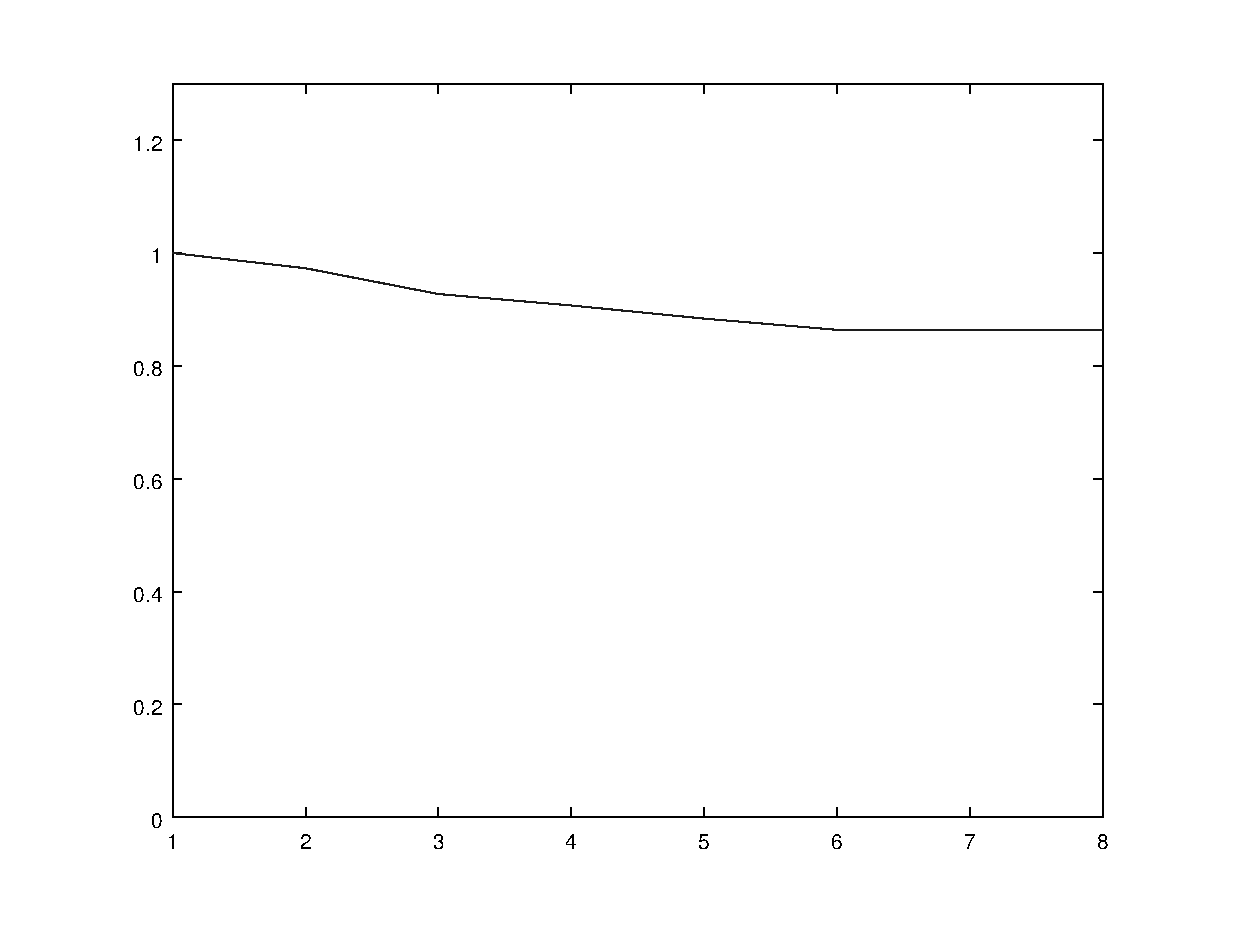
\includegraphics[width=0.8\columnwidth]{images/graph1.eps}
\caption{Departure factor for each frame in the test 1.}
\label{fig:res_graph1}
\end{figure}
The Fig. \ref{fig:res_graph1v} shows the velocity of departure factor
to a value $d_0=1$ and a $\Delta t=1$. It is easy to see that the variation,
between frames, of departure factor is very small when compared with 1, 
having a mean departure velocity of $-0.017020$. This imply a mean approach of $1.7\%$ of $d_0$
by frame.
\begin{figure}[!hbt]
\centering
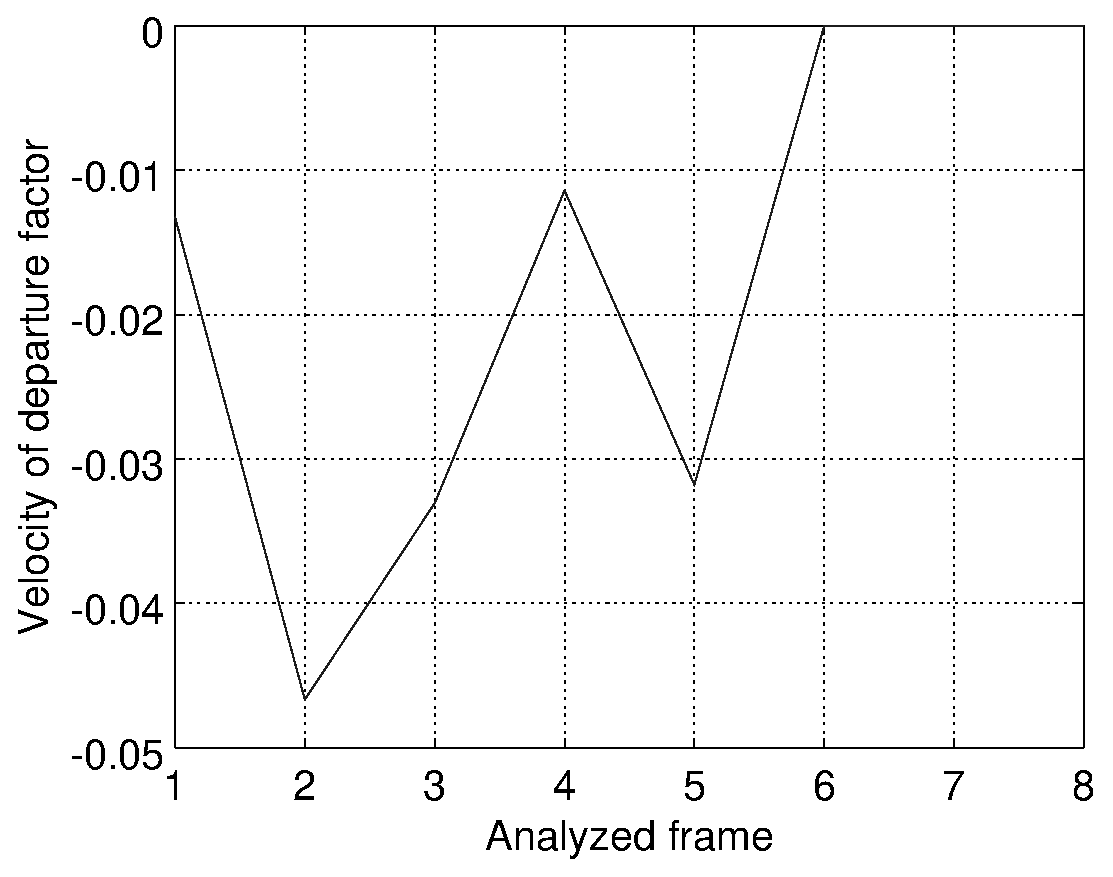
\includegraphics[width=0.8\columnwidth]{images/graph1v.eps}
\caption{Velocity of departure factor for each frame in the test 1.}
\label{fig:res_graph1v}
\end{figure}


In the second test, we prove the functionality of algorithm in 3D. 
The program compares the images and calculate the departure factor 
based on the area of object. The Fig. \ref{fig:target} demonstrates the 
tracking from initial at the final position of target.
\begin{figure}[!hbt]
\centering
  \subfloat[]{\label{fig:targeinit} \includegraphics[width=.48\columnwidth]{images/images/351.jpg}}
  \subfloat[]{\label{fig:targeend} \includegraphics[width=.48\columnwidth]{images/images/450.jpg}}
  \caption{The object in (a) is the initial position and its area is 
  fewer than the figure in (b), which is in final position. 
  The factor is calculate dividing both areas.}
  \label{fig:target}
\end{figure}
The vector that describes the movement of object is showed. 
We can observe the significant increase in area of vehicle. So, it 
contributes, directly, with the departure factor.

\begin{figure}[!hbt]
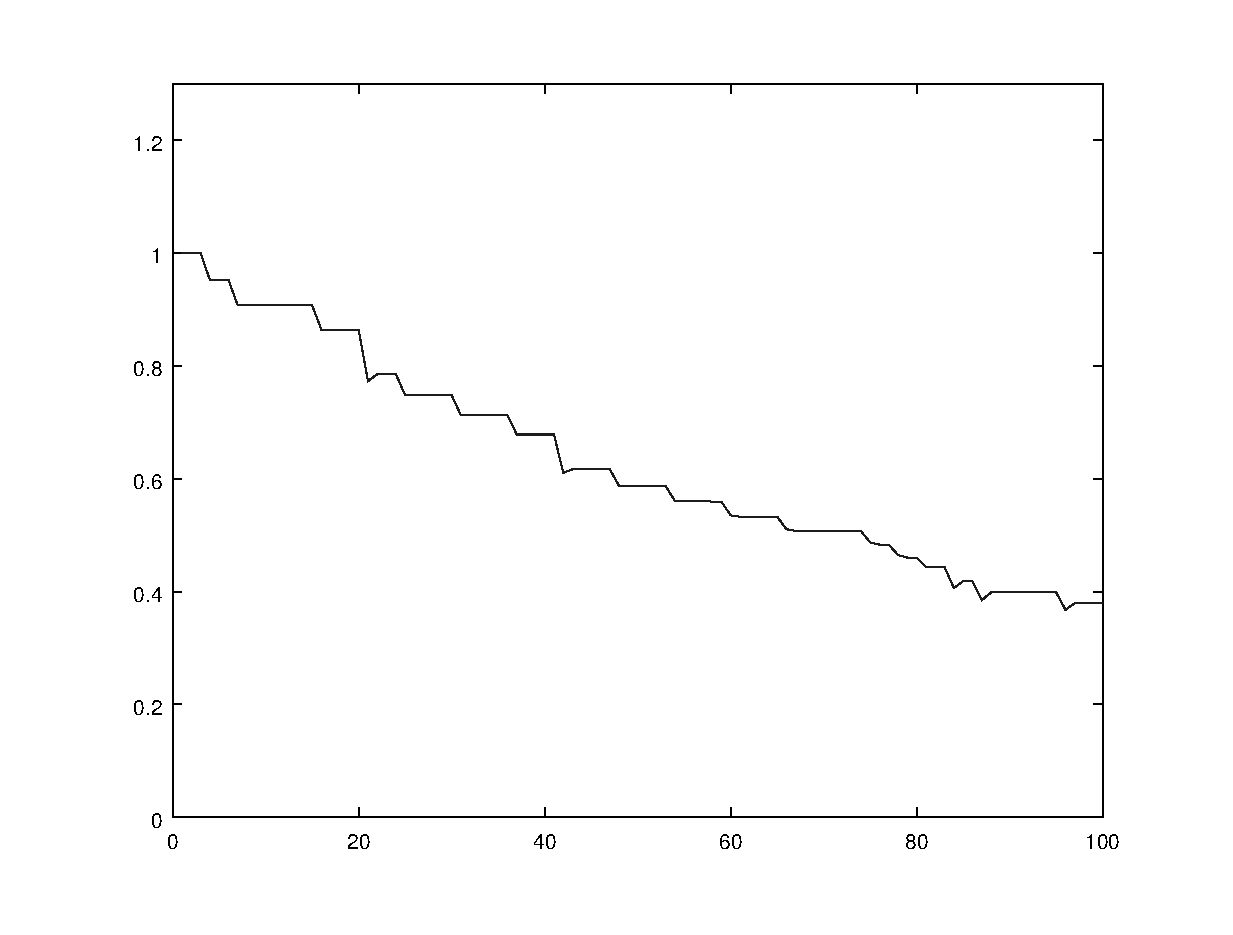
\includegraphics[width=\columnwidth]{images/graph2.eps}
\caption{Departure factor for each frame in the test 2.}
\label{fig:res_graph2}
\end{figure}
The graphic of Fig. \ref{fig:res_graph2} with the departure factor in each frame
of test 2, could be interpreted as position per time, 
because that the departure factor describes the relative target position.
Thus in the first image the analyzed object is at a distance $d$ and in the last frame
the object is at a distance of $40\%$ of $d$.



One application using tracking and departure factor is 
related with risk of collision. 
It is possible estimate how fast any object is departing,
then, if the factor tends to zero or if it changes to values 
fewer every time, probably, there is a high risk of collision.


